%\section{Libvina: A template library}
%\label{sec:lib}

%We implement a prototype template library, libvina,  to demonstrate
%our approach.

\section{Adaption for Libvina}
\label{sec:adaption}

Programmers who apply our approach need to customize their source code
to utilize libvina. Technically speaking, we provide a group of \emph{concepts}
in libvina to support transformations and expect programmrs to \textit{model} our
template classes~\cite{tempmetaprog}. 

\subsection{Function Wrapper}

Function wrapper is an idiom in libvina. Our approach needs to manipulate
template functions according to their template arguments. However, a
template function is unaddressable until it is
instantiated. Thus programmers have to bind their template functions
to entries of classes.  Either static function or call operator
fuctions is approachable, but there is tradeoff to consider.
Static function need to predefine naming convention. 
For example, \code{TF\_hierarchy} use names \code{inner} and
\code{leaf} to call back. Call operator has unique form to invoke, so we leave it
as user interface, at expense of runtime
cost~\footnote{C++ does not allow overload call operator using static
  function, therefore we have to generate an object to call it.}. Line 14
of \reffig{sgemm} is the case.

%Another restrict of function is that our
%template can only handle fixed form of function. \textit{i.e.} the
%function signature is triple form\footnote{function form: void (ARG0, ARG1,
% RESULT).We expect template alias in C++0x can releave this
%  retrict. } and parameter passing semantics is CBVR~\cite{dragonbook}.

\subsection{Adaption for TF\_hierarchy}

Line 6$\sim$10 of \reffig{sgemm} is adaption for \code{TF\_hierarchy}. Line 10
defines the type of task for \code{SGEMM}. It is used as
the template parameter \code{TASK} for \code{TF\_hierarchy} class. PRED template
parameter at line 11 is a predicate and \code{TF\_hierarchy} class will
evaluate it using \code{ARG0} and \code{ARG1}. Line 18 calls customized TF class after dividing
task. According to template argument, TF class determines whether
reenter the entry inner at line 22 or terminate at leaf at
line 45. Function leaf performs computation. \reffig{hierarchy} illustrates
instantiation process of \code{TF\_hierarchy} and \reffig{mmexample} is
execution after transformation. The figure depicts the case K is 2.

\begin{figure}[hpt]
  \includegraphics[width=3.5in]{../algo}
  \caption{Instantiation process of \code{TF\_hierarchy}. The predicate is a template
class, which is evaluted using \code{TASK}'s parameters.}
  \label{fig:hierarchy}
\end{figure}

%for sequoia's programming mode: 
%define recursive rules 
% for stream 's programming model:

\subsection{Adaption for TF\_pipeline}

To leverage \code{TF\_pipeline}, programmers have to provide a full
specialization template class. This is because \code{TF\_pipeline}
only synthesizes functions and executes them in order, but does not
know how to process the output.
\todo{A full specialization of TF\_pipeline defines this behavior and is called at last.
For example in \reffig{pipe}, line 2$\sim$21 is the case.}
Static entry at line 13 serves \code{TF\_pipeline} class. We spawn a thread to handle with the output 
from the previous stage. Line 24$\sim$31 is a usage of \code{TF\_pipeline} with 4
standalone functions. All the stages including our customized one are
threads. It is noteworthy that each immediate stage, e.g.,
\code{translate$<$Frn2Spn$>$}, has to follow type interfaces and
define dependences. In \textit{lang\_pipe} case, we use \code{ReadViewMT} and
\code{WriteViewMT} to synchronize two adjacent stages.
%Asynchronous signals in ViewMTs provoke waiting stages and are used to mimic data-flow diagram.
As \reffig{viewmt} showing, \code{WriteViewMT} of a previous stage signals the
\code{ReadViewMT} of the next stage that data is ready.

\begin{figure}[tp]
  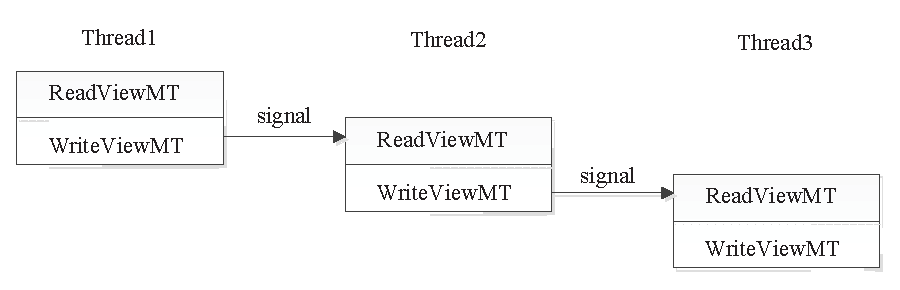
\includegraphics[width=3.1in]{../viewmt}
  \caption{Pipeline processing using ViewMTs. Access to a \code{ReadViewMT} is
  blocking until it is signaled. A stage sets its signal of \code{WriteViewMT}
after data processing is complete.}
  \label{fig:viewmt}
\end{figure}

%end of section.
